\documentclass[1p]{elsarticle_modified}
%\bibliographystyle{elsarticle-num}

%\usepackage[colorlinks]{hyperref}
%\usepackage{abbrmath_seonhwa} %\Abb, \Ascr, \Acal ,\Abf, \Afrak
\usepackage{amsfonts}
\usepackage{amssymb}
\usepackage{amsmath}
\usepackage{amsthm}
\usepackage{scalefnt}
\usepackage{amsbsy}
\usepackage{kotex}
\usepackage{caption}
\usepackage{subfig}
\usepackage{color}
\usepackage{graphicx}
\usepackage{xcolor} %% white, black, red, green, blue, cyan, magenta, yellow
\usepackage{float}
\usepackage{setspace}
\usepackage{hyperref}

\usepackage{tikz}
\usetikzlibrary{arrows}

\usepackage{multirow}
\usepackage{array} % fixed length table
\usepackage{hhline}

%%%%%%%%%%%%%%%%%%%%%
\makeatletter
\renewcommand*\env@matrix[1][\arraystretch]{%
	\edef\arraystretch{#1}%
	\hskip -\arraycolsep
	\let\@ifnextchar\new@ifnextchar
	\array{*\c@MaxMatrixCols c}}
\makeatother %https://tex.stackexchange.com/questions/14071/how-can-i-increase-the-line-spacing-in-a-matrix
%%%%%%%%%%%%%%%

\usepackage[normalem]{ulem}

\newcommand{\msout}[1]{\ifmmode\text{\sout{\ensuremath{#1}}}\else\sout{#1}\fi}
%SOURCE: \msout is \stkout macro in https://tex.stackexchange.com/questions/20609/strikeout-in-math-mode

\newcommand{\cancel}[1]{
	\ifmmode
	{\color{red}\msout{#1}}
	\else
	{\color{red}\sout{#1}}
	\fi
}

\newcommand{\add}[1]{
	{\color{blue}\uwave{#1}}
}

\newcommand{\replace}[2]{
	\ifmmode
	{\color{red}\msout{#1}}{\color{blue}\uwave{#2}}
	\else
	{\color{red}\sout{#1}}{\color{blue}\uwave{#2}}
	\fi
}

\newcommand{\Sol}{\mathcal{S}} %segment
\newcommand{\D}{D} %diagram
\newcommand{\A}{\mathcal{A}} %arc


%%%%%%%%%%%%%%%%%%%%%%%%%%%%%5 test

\def\sl{\operatorname{\textup{SL}}(2,\Cbb)}
\def\psl{\operatorname{\textup{PSL}}(2,\Cbb)}
\def\quan{\mkern 1mu \triangleright \mkern 1mu}

\theoremstyle{definition}
\newtheorem{thm}{Theorem}[section]
\newtheorem{prop}[thm]{Proposition}
\newtheorem{lem}[thm]{Lemma}
\newtheorem{ques}[thm]{Question}
\newtheorem{cor}[thm]{Corollary}
\newtheorem{defn}[thm]{Definition}
\newtheorem{exam}[thm]{Example}
\newtheorem{rmk}[thm]{Remark}
\newtheorem{alg}[thm]{Algorithm}

\newcommand{\I}{\sqrt{-1}}
\begin{document}

%\begin{frontmatter}
%
%\title{Boundary parabolic representations of knots up to 8 crossings}
%
%%% Group authors per affiliation:
%\author{Yunhi Cho} 
%\address{Department of Mathematics, University of Seoul, Seoul, Korea}
%\ead{yhcho@uos.ac.kr}
%
%
%\author{Seonhwa Kim} %\fnref{s_kim}}
%\address{Center for Geometry and Physics, Institute for Basic Science, Pohang, 37673, Korea}
%\ead{ryeona17@ibs.re.kr}
%
%\author{Hyuk Kim}
%\address{Department of Mathematical Sciences, Seoul National University, Seoul 08826, Korea}
%\ead{hyukkim@snu.ac.kr}
%
%\author{Seokbeom Yoon}
%\address{Department of Mathematical Sciences, Seoul National University, Seoul, 08826,  Korea}
%\ead{sbyoon15@snu.ac.kr}
%
%\begin{abstract}
%We find all boundary parabolic representation of knots up to 8 crossings.
%
%\end{abstract}
%\begin{keyword}
%    \MSC[2010] 57M25 
%\end{keyword}
%
%\end{frontmatter}

%\linenumbers
%\tableofcontents
%
\newcommand\colored[1]{\textcolor{white}{\rule[-0.35ex]{0.8em}{1.4ex}}\kern-0.8em\color{red} #1}%
%\newcommand\colored[1]{\textcolor{white}{ #1}\kern-2.17ex	\textcolor{white}{ #1}\kern-1.81ex	\textcolor{white}{ #1}\kern-2.15ex\color{red}#1	}

{\Large $\underline{11a_{354}~(K11a_{354})}$}

\setlength{\tabcolsep}{10pt}
\renewcommand{\arraystretch}{1.6}
\vspace{1cm}\begin{tabular}{m{100pt}>{\centering\arraybackslash}m{274pt}}
\multirow{5}{120pt}{
	\centering
	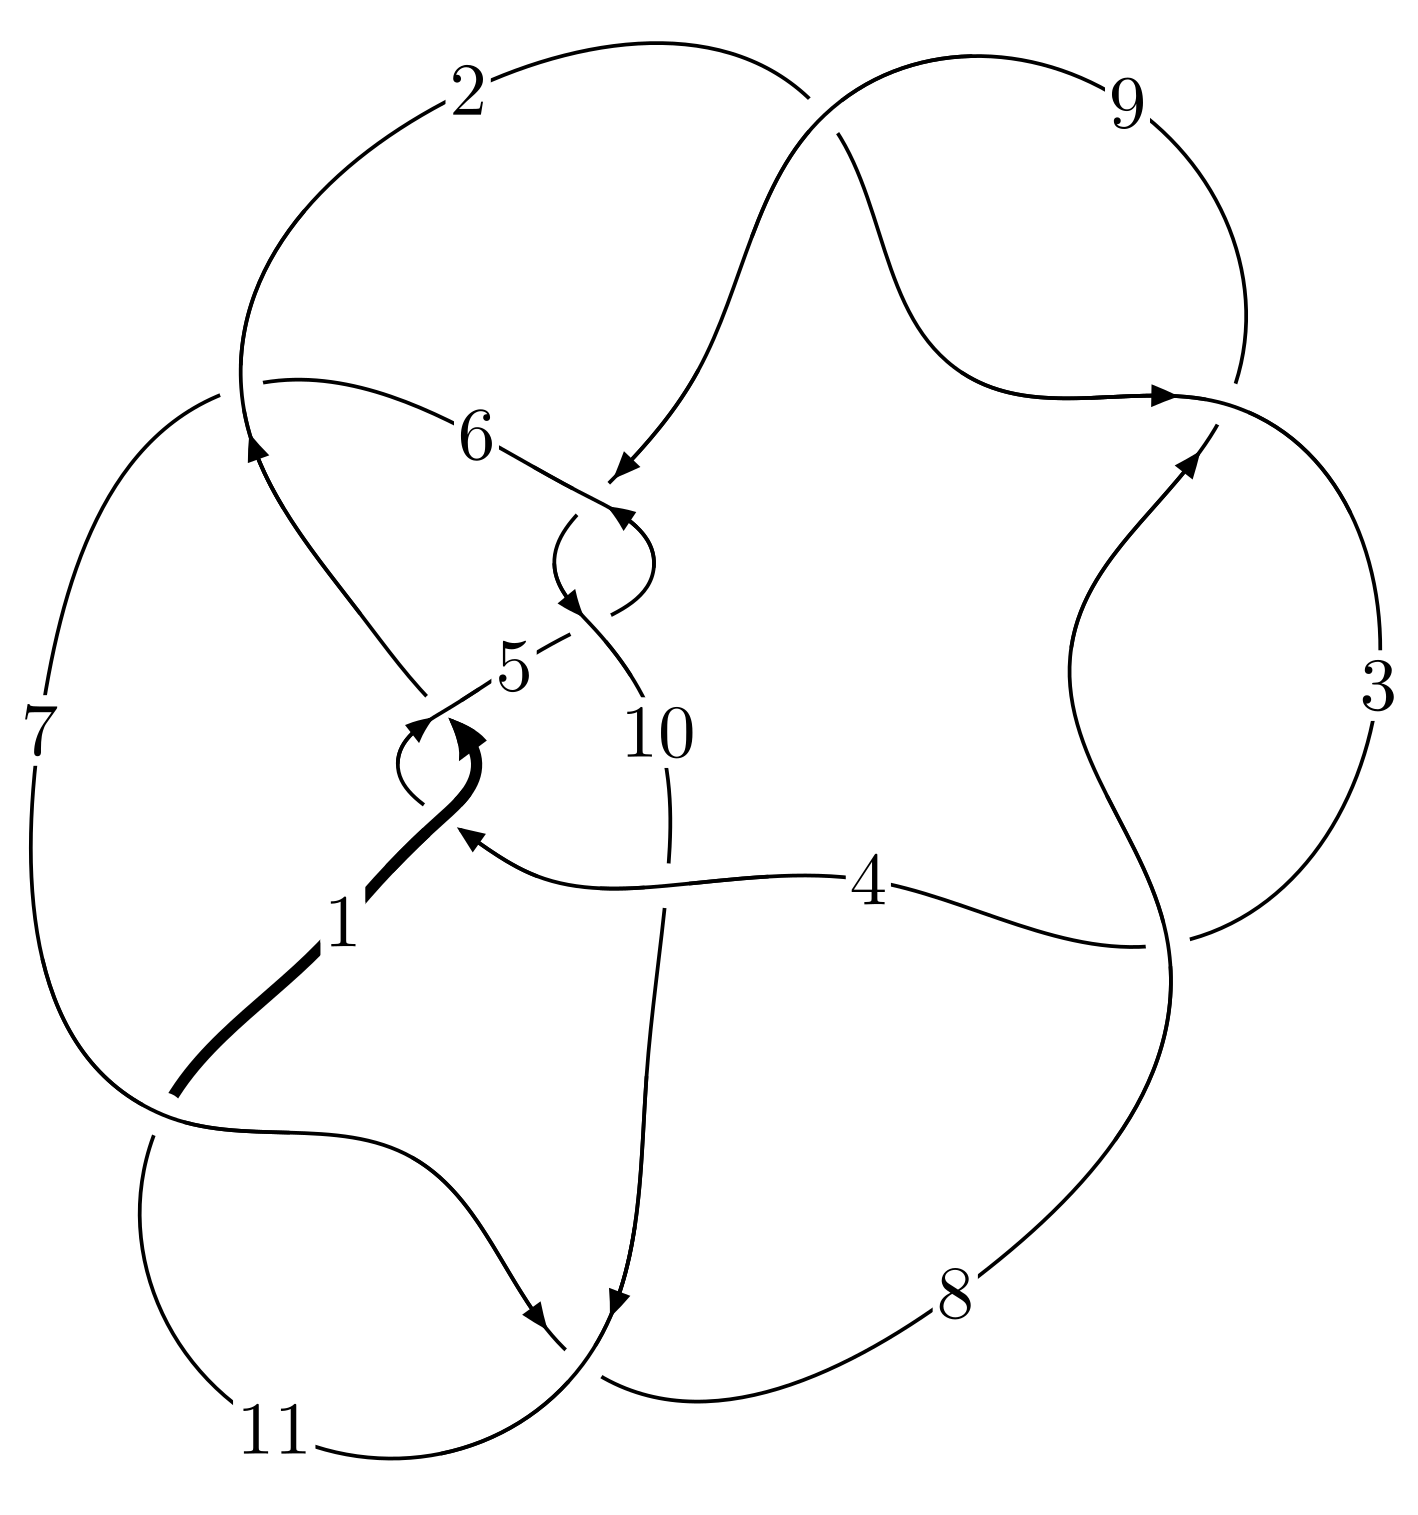
\includegraphics[width=112pt]{../../../GIT/diagram.site/Diagrams/png/603_11a_354.png}\\
\ \ \ A knot diagram\footnotemark}&
\allowdisplaybreaks
\textbf{Linearized knot diagam} \\
\cline{2-2}
 &
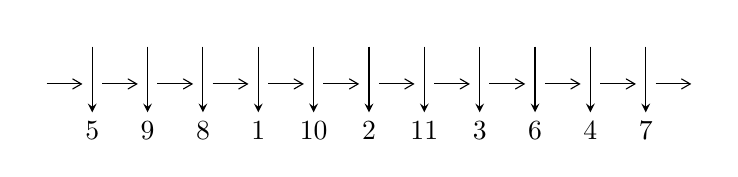
\begin{tikzpicture}[x=20pt, y=17pt]
	% nodes
	\node (C0) at (0, 0) {};
	\node (C1) at (1, 0) {};
	\node (C1U) at (1, +1) {};
	\node (C1D) at (1, -1) {5};

	\node (C2) at (2, 0) {};
	\node (C2U) at (2, +1) {};
	\node (C2D) at (2, -1) {9};

	\node (C3) at (3, 0) {};
	\node (C3U) at (3, +1) {};
	\node (C3D) at (3, -1) {8};

	\node (C4) at (4, 0) {};
	\node (C4U) at (4, +1) {};
	\node (C4D) at (4, -1) {1};

	\node (C5) at (5, 0) {};
	\node (C5U) at (5, +1) {};
	\node (C5D) at (5, -1) {10};

	\node (C6) at (6, 0) {};
	\node (C6U) at (6, +1) {};
	\node (C6D) at (6, -1) {2};

	\node (C7) at (7, 0) {};
	\node (C7U) at (7, +1) {};
	\node (C7D) at (7, -1) {11};

	\node (C8) at (8, 0) {};
	\node (C8U) at (8, +1) {};
	\node (C8D) at (8, -1) {3};

	\node (C9) at (9, 0) {};
	\node (C9U) at (9, +1) {};
	\node (C9D) at (9, -1) {6};

	\node (C10) at (10, 0) {};
	\node (C10U) at (10, +1) {};
	\node (C10D) at (10, -1) {4};

	\node (C11) at (11, 0) {};
	\node (C11U) at (11, +1) {};
	\node (C11D) at (11, -1) {7};
	\node (C12) at (12, 0) {};

	% arrows
	\draw[->,>={angle 60}]
	(C0) edge (C1) (C1) edge (C2) (C2) edge (C3) (C3) edge (C4) (C4) edge (C5) (C5) edge (C6) (C6) edge (C7) (C7) edge (C8) (C8) edge (C9) (C9) edge (C10) (C10) edge (C11) (C11) edge (C12) ;	\draw[->,>=stealth]
	(C1U) edge (C1D) (C2U) edge (C2D) (C3U) edge (C3D) (C4U) edge (C4D) (C5U) edge (C5D) (C6U) edge (C6D) (C7U) edge (C7D) (C8U) edge (C8D) (C9U) edge (C9D) (C10U) edge (C10D) (C11U) edge (C11D) ;
	\end{tikzpicture} \\
\hhline{~~} \\& 
\textbf{Solving Sequence} \\ \cline{2-2} 
 &
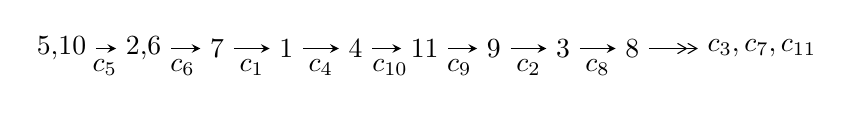
\begin{tikzpicture}[x=25pt, y=7pt]
	% node
	\node (A0) at (-1/8, 0) {5,10};
	\node (A1) at (17/16, 0) {2,6};
	\node (A2) at (17/8, 0) {7};
	\node (A3) at (25/8, 0) {1};
	\node (A4) at (33/8, 0) {4};
	\node (A5) at (41/8, 0) {11};
	\node (A6) at (49/8, 0) {9};
	\node (A7) at (57/8, 0) {3};
	\node (A8) at (65/8, 0) {8};
	\node (C1) at (1/2, -1) {$c_{5}$};
	\node (C2) at (13/8, -1) {$c_{6}$};
	\node (C3) at (21/8, -1) {$c_{1}$};
	\node (C4) at (29/8, -1) {$c_{4}$};
	\node (C5) at (37/8, -1) {$c_{10}$};
	\node (C6) at (45/8, -1) {$c_{9}$};
	\node (C7) at (53/8, -1) {$c_{2}$};
	\node (C8) at (61/8, -1) {$c_{8}$};
	\node (A9) at (10, 0) {$c_{3},c_{7},c_{11}$};

	% edge
	\draw[->,>=stealth]	
	(A0) edge (A1) (A1) edge (A2) (A2) edge (A3) (A3) edge (A4) (A4) edge (A5) (A5) edge (A6) (A6) edge (A7) (A7) edge (A8) ;
	\draw[->>,>={angle 60}]	
	(A8) edge (A9);
\end{tikzpicture} \\ 

\end{tabular} \\

\footnotetext{
The image of knot diagram is generated by the software ``\textbf{Draw programme}" developed by Andrew Bartholomew(\url{http://www.layer8.co.uk/maths/draw/index.htm\#Running-draw}), where we modified some parts for our purpose(\url{https://github.com/CATsTAILs/LinksPainter}).
}\phantom \\ \newline 
\centering \textbf{Ideals for irreducible components\footnotemark of $X_{\text{par}}$} 
 
\begin{align*}
I^u_{1}&=\langle 
-160922417 u^{20}-82767962 u^{19}+\cdots+2637274048 b+1724364181,\\
\phantom{I^u_{1}}&\phantom{= \langle  }1172455205 u^{20}+3315332618 u^{19}+\cdots+15823644288 a-17023392209,\;u^{21}+u^{20}+\cdots- u-3\rangle \\
I^u_{2}&=\langle 
3.10404\times10^{24} u^{33}-6.92641\times10^{24} u^{32}+\cdots+3.33278\times10^{25} b+3.58251\times10^{25},\\
\phantom{I^u_{2}}&\phantom{= \langle  }2.34878\times10^{26} u^{33}-6.49522\times10^{26} u^{32}+\cdots+9.99835\times10^{25} a-2.61013\times10^{26},\;u^{34}-3 u^{33}+\cdots-8 u+1\rangle \\
I^u_{3}&=\langle 
b+1,\;2 a+1,\;u-1\rangle \\
I^u_{4}&=\langle 
b-1,\;4 a^2-4 a+3,\;u+1\rangle \\
\\
\end{align*}
\raggedright * 4 irreducible components of $\dim_{\mathbb{C}}=0$, with total 58 representations.\\
\footnotetext{All coefficients of polynomials are rational numbers. But the coefficients are sometimes approximated in decimal forms when there is not enough margin.}
\newpage
\renewcommand{\arraystretch}{1}
\centering \section*{I. $I^u_{1}= \langle -1.61\times10^{8} u^{20}-8.28\times10^{7} u^{19}+\cdots+2.64\times10^{9} b+1.72\times10^{9},\;1.17\times10^{9} u^{20}+3.32\times10^{9} u^{19}+\cdots+1.58\times10^{10} a-1.70\times10^{10},\;u^{21}+u^{20}+\cdots- u-3 \rangle$}
\flushleft \textbf{(i) Arc colorings}\\
\begin{tabular}{m{7pt} m{180pt} m{7pt} m{180pt} }
\flushright $a_{5}=$&$\begin{pmatrix}1\\0\end{pmatrix}$ \\
\flushright $a_{10}=$&$\begin{pmatrix}0\\u\end{pmatrix}$ \\
\flushright $a_{2}=$&$\begin{pmatrix}-0.0740951 u^{20}-0.209518 u^{19}+\cdots-3.81221 u+1.07582\\0.0610185 u^{20}+0.0313839 u^{19}+\cdots+1.11500 u-0.653843\end{pmatrix}$ \\
\flushright $a_{6}=$&$\begin{pmatrix}1\\u^2\end{pmatrix}$ \\
\flushright $a_{7}=$&$\begin{pmatrix}-0.197971 u^{20}-0.0494518 u^{19}+\cdots+0.314954 u+1.35005\\0.165057 u^{20}-0.0143368 u^{19}+\cdots-0.408900 u+0.0392300\end{pmatrix}$ \\
\flushright $a_{1}=$&$\begin{pmatrix}-0.0130767 u^{20}-0.178134 u^{19}+\cdots-2.69722 u+0.421977\\0.0610185 u^{20}+0.0313839 u^{19}+\cdots+1.11500 u-0.653843\end{pmatrix}$ \\
\flushright $a_{4}=$&$\begin{pmatrix}-0.0825253 u^{20}-0.112909 u^{19}+\cdots-0.258326 u+1.55523\\-0.208288 u^{20}-0.526602 u^{19}+\cdots+1.07412 u+0.824561\end{pmatrix}$ \\
\flushright $a_{11}=$&$\begin{pmatrix}0.135443 u^{20}-0.0407053 u^{19}+\cdots-1.54514 u-0.171937\\-0.118375 u^{20}-0.208719 u^{19}+\cdots+1.31928 u-0.158672\end{pmatrix}$ \\
\flushright $a_{9}=$&$\begin{pmatrix}u\\u^3+u\end{pmatrix}$ \\
\flushright $a_{3}=$&$\begin{pmatrix}-0.00777699 u^{20}-0.204864 u^{19}+\cdots-4.09651 u+0.616331\\0.242228 u^{20}+0.162054 u^{19}+\cdots+0.967988 u-1.29833\end{pmatrix}$ \\
\flushright $a_{8}=$&$\begin{pmatrix}-0.374119 u^{20}-0.144655 u^{19}+\cdots+0.278460 u+1.75638\\0.0747139 u^{20}+0.125515 u^{19}+\cdots-0.685947 u-0.315896\end{pmatrix}$\\ \flushright $a_{8}=$&$\begin{pmatrix}-0.374119 u^{20}-0.144655 u^{19}+\cdots+0.278460 u+1.75638\\0.0747139 u^{20}+0.125515 u^{19}+\cdots-0.685947 u-0.315896\end{pmatrix}$\\&\end{tabular}
\flushleft \textbf{(ii) Obstruction class $= -1$}\\~\\
\flushleft \textbf{(iii) Cusp Shapes $= \frac{637817299}{659318512} u^{20}+\frac{458613173}{659318512} u^{19}+\cdots-\frac{13858087997}{659318512} u-\frac{901043607}{82414814}$}\\~\\
\newpage\renewcommand{\arraystretch}{1}
\flushleft \textbf{(iv) u-Polynomials at the component}\newline \\
\begin{tabular}{m{50pt}|m{274pt}}
Crossings & \hspace{64pt}u-Polynomials at each crossing \\
\hline $$\begin{aligned}c_{1},c_{4}\end{aligned}$$&$\begin{aligned}
&u^{21}-6 u^{19}+\cdots+57 u+24
\end{aligned}$\\
\hline $$\begin{aligned}c_{2},c_{3},c_{8}\end{aligned}$$&$\begin{aligned}
&u^{21}-3 u^{20}+\cdots-24 u+8
\end{aligned}$\\
\hline $$\begin{aligned}c_{5},c_{7},c_{9}\\c_{11}\end{aligned}$$&$\begin{aligned}
&u^{21}- u^{20}+\cdots- u+3
\end{aligned}$\\
\hline $$\begin{aligned}c_{6},c_{10}\end{aligned}$$&$\begin{aligned}
&8(8 u^{21}-4 u^{20}+\cdots-2 u+4)
\end{aligned}$\\
\hline
\end{tabular}\\~\\
\newpage\renewcommand{\arraystretch}{1}
\flushleft \textbf{(v) Riley Polynomials at the component}\newline \\
\begin{tabular}{m{50pt}|m{274pt}}
Crossings & \hspace{64pt}Riley Polynomials at each crossing \\
\hline $$\begin{aligned}c_{1},c_{4}\end{aligned}$$&$\begin{aligned}
&y^{21}-12 y^{20}+\cdots+13233 y-576
\end{aligned}$\\
\hline $$\begin{aligned}c_{2},c_{3},c_{8}\end{aligned}$$&$\begin{aligned}
&y^{21}+23 y^{20}+\cdots+96 y-64
\end{aligned}$\\
\hline $$\begin{aligned}c_{5},c_{7},c_{9}\\c_{11}\end{aligned}$$&$\begin{aligned}
&y^{21}+11 y^{20}+\cdots+85 y-9
\end{aligned}$\\
\hline $$\begin{aligned}c_{6},c_{10}\end{aligned}$$&$\begin{aligned}
&64(64 y^{21}+656 y^{20}+\cdots+60 y-16)
\end{aligned}$\\
\hline
\end{tabular}\\~\\
\newpage\flushleft \textbf{(vi) Complex Volumes and Cusp Shapes}
$$\begin{array}{c|c|c}  
\text{Solutions to }I^u_{1}& \I (\text{vol} + \sqrt{-1}CS) & \text{Cusp shape}\\
 \hline 
\begin{aligned}
u &= \phantom{-}1.090880 + 0.306968 I \\
a &= -0.388613 + 0.046984 I \\
b &= -1.011870 + 0.167863 I\end{aligned}
 & -3.50254 + 0.45372 I & -13.2351 - 10.9889 I \\ \hline\begin{aligned}
u &= \phantom{-}1.090880 - 0.306968 I \\
a &= -0.388613 - 0.046984 I \\
b &= -1.011870 - 0.167863 I\end{aligned}
 & -3.50254 - 0.45372 I & -13.2351 + 10.9889 I \\ \hline\begin{aligned}
u &= \phantom{-}0.300491 + 1.132360 I \\
a &= -0.48749 - 1.67733 I \\
b &= \phantom{-}1.27655 + 0.93600 I\end{aligned}
 & \phantom{-}2.01539 - 5.30911 I & -6.93058 + 7.06093 I \\ \hline\begin{aligned}
u &= \phantom{-}0.300491 - 1.132360 I \\
a &= -0.48749 + 1.67733 I \\
b &= \phantom{-}1.27655 - 0.93600 I\end{aligned}
 & \phantom{-}2.01539 + 5.30911 I & -6.93058 - 7.06093 I \\ \hline\begin{aligned}
u &= \phantom{-}0.059914 + 1.172390 I \\
a &= \phantom{-}1.13290 - 0.84676 I \\
b &= -1.89114 + 0.74167 I\end{aligned}
 & \phantom{-}8.68556 - 1.36021 I & \phantom{-}3.27021 + 3.85751 I \\ \hline\begin{aligned}
u &= \phantom{-}0.059914 - 1.172390 I \\
a &= \phantom{-}1.13290 + 0.84676 I \\
b &= -1.89114 - 0.74167 I\end{aligned}
 & \phantom{-}8.68556 + 1.36021 I & \phantom{-}3.27021 - 3.85751 I \\ \hline\begin{aligned}
u &= -0.173596 + 1.178810 I \\
a &= \phantom{-}0.45364 + 1.66491 I \\
b &= -0.33964 - 1.52106 I\end{aligned}
 & \phantom{-}6.35701 + 3.86289 I & -1.42698 - 7.24526 I \\ \hline\begin{aligned}
u &= -0.173596 - 1.178810 I \\
a &= \phantom{-}0.45364 - 1.66491 I \\
b &= -0.33964 + 1.52106 I\end{aligned}
 & \phantom{-}6.35701 - 3.86289 I & -1.42698 + 7.24526 I \\ \hline\begin{aligned}
u &= -0.533873 + 0.533126 I \\
a &= \phantom{-}0.131827 + 0.649526 I \\
b &= \phantom{-}1.259740 + 0.049663 I\end{aligned}
 & -2.36275 + 1.38248 I & -10.93113 - 5.35701 I \\ \hline\begin{aligned}
u &= -0.533873 - 0.533126 I \\
a &= \phantom{-}0.131827 - 0.649526 I \\
b &= \phantom{-}1.259740 - 0.049663 I\end{aligned}
 & -2.36275 - 1.38248 I & -10.93113 + 5.35701 I\\
 \hline 
 \end{array}$$\newpage$$\begin{array}{c|c|c}  
\text{Solutions to }I^u_{1}& \I (\text{vol} + \sqrt{-1}CS) & \text{Cusp shape}\\
 \hline 
\begin{aligned}
u &= -0.485617 + 1.267790 I \\
a &= \phantom{-}0.17265 - 1.58270 I \\
b &= -1.29660 + 0.72895 I\end{aligned}
 & \phantom{-}3.28365 + 11.20830 I & -7.47113 - 8.56307 I \\ \hline\begin{aligned}
u &= -0.485617 - 1.267790 I \\
a &= \phantom{-}0.17265 + 1.58270 I \\
b &= -1.29660 - 0.72895 I\end{aligned}
 & \phantom{-}3.28365 - 11.20830 I & -7.47113 + 8.56307 I \\ \hline\begin{aligned}
u &= \phantom{-}0.37790 + 1.38499 I \\
a &= -0.392046 + 1.240810 I \\
b &= \phantom{-}0.173107 - 1.254650 I\end{aligned}
 & \phantom{-}14.7040 - 8.5355 I & -2.42060 + 4.78360 I \\ \hline\begin{aligned}
u &= \phantom{-}0.37790 - 1.38499 I \\
a &= -0.392046 - 1.240810 I \\
b &= \phantom{-}0.173107 + 1.254650 I\end{aligned}
 & \phantom{-}14.7040 + 8.5355 I & -2.42060 - 4.78360 I \\ \hline\begin{aligned}
u &= -0.409786 + 0.332736 I \\
a &= \phantom{-}1.34718 - 1.22922 I \\
b &= -0.508583 + 0.245922 I\end{aligned}
 & \phantom{-}3.45120 + 1.15767 I & -7.19855 - 5.90528 I \\ \hline\begin{aligned}
u &= -0.409786 - 0.332736 I \\
a &= \phantom{-}1.34718 + 1.22922 I \\
b &= -0.508583 - 0.245922 I\end{aligned}
 & \phantom{-}3.45120 - 1.15767 I & -7.19855 + 5.90528 I \\ \hline\begin{aligned}
u &= -1.44772 + 0.30988 I \\
a &= \phantom{-}0.380476 - 0.106586 I \\
b &= \phantom{-}0.868563 + 0.334615 I\end{aligned}
 & \phantom{-}2.63271 - 1.46369 I & -5.79825 + 4.59200 I \\ \hline\begin{aligned}
u &= -1.44772 - 0.30988 I \\
a &= \phantom{-}0.380476 + 0.106586 I \\
b &= \phantom{-}0.868563 - 0.334615 I\end{aligned}
 & \phantom{-}2.63271 + 1.46369 I & -5.79825 - 4.59200 I \\ \hline\begin{aligned}
u &= \phantom{-}0.57781 + 1.39987 I \\
a &= -0.00890 - 1.47507 I \\
b &= \phantom{-}1.33922 + 0.65997 I\end{aligned}
 & \phantom{-}11.0553 - 15.1817 I & -5.60482 + 7.58890 I \\ \hline\begin{aligned}
u &= \phantom{-}0.57781 - 1.39987 I \\
a &= -0.00890 + 1.47507 I \\
b &= \phantom{-}1.33922 - 0.65997 I\end{aligned}
 & \phantom{-}11.0553 + 15.1817 I & -5.60482 - 7.58890 I\\
 \hline 
 \end{array}$$\newpage$$\begin{array}{c|c|c}  
\text{Solutions to }I^u_{1}& \I (\text{vol} + \sqrt{-1}CS) & \text{Cusp shape}\\
 \hline 
\begin{aligned}
u &= \phantom{-}0.287195\phantom{ +0.000000I} \\
a &= -0.849896\phantom{ +0.000000I} \\
b &= \phantom{-}0.261262\phantom{ +0.000000I}\end{aligned}
 & -0.522581\phantom{ +0.000000I} & -19.0060\phantom{ +0.000000I}\\
 \hline 
 \end{array}$$\newpage\newpage\renewcommand{\arraystretch}{1}
\centering \section*{II. $I^u_{2}= \langle 3.10\times10^{24} u^{33}-6.93\times10^{24} u^{32}+\cdots+3.33\times10^{25} b+3.58\times10^{25},\;2.35\times10^{26} u^{33}-6.50\times10^{26} u^{32}+\cdots+1.00\times10^{26} a-2.61\times10^{26},\;u^{34}-3 u^{33}+\cdots-8 u+1 \rangle$}
\flushleft \textbf{(i) Arc colorings}\\
\begin{tabular}{m{7pt} m{180pt} m{7pt} m{180pt} }
\flushright $a_{5}=$&$\begin{pmatrix}1\\0\end{pmatrix}$ \\
\flushright $a_{10}=$&$\begin{pmatrix}0\\u\end{pmatrix}$ \\
\flushright $a_{2}=$&$\begin{pmatrix}-2.34917 u^{33}+6.49629 u^{32}+\cdots-50.6654 u+2.61056\\-0.0931366 u^{33}+0.207827 u^{32}+\cdots-1.02591 u-1.07493\end{pmatrix}$ \\
\flushright $a_{6}=$&$\begin{pmatrix}1\\u^2\end{pmatrix}$ \\
\flushright $a_{7}=$&$\begin{pmatrix}1.80446 u^{33}-4.85974 u^{32}+\cdots+35.4986 u+5.80588\\-0.547249 u^{33}+1.50787 u^{32}+\cdots-10.1466 u+3.14923\end{pmatrix}$ \\
\flushright $a_{1}=$&$\begin{pmatrix}-2.44231 u^{33}+6.70412 u^{32}+\cdots-51.6914 u+1.53563\\-0.0931366 u^{33}+0.207827 u^{32}+\cdots-1.02591 u-1.07493\end{pmatrix}$ \\
\flushright $a_{4}=$&$\begin{pmatrix}-1.62724 u^{33}+4.23174 u^{32}+\cdots-36.5972 u-2.57013\\0.387178 u^{33}-1.14075 u^{32}+\cdots+6.79493 u-2.47847\end{pmatrix}$ \\
\flushright $a_{11}=$&$\begin{pmatrix}-6.82156 u^{33}+19.3458 u^{32}+\cdots-168.898 u+23.4185\\-0.665031 u^{33}+1.70903 u^{32}+\cdots-14.3783 u+0.0625691\end{pmatrix}$ \\
\flushright $a_{9}=$&$\begin{pmatrix}u\\u^3+u\end{pmatrix}$ \\
\flushright $a_{3}=$&$\begin{pmatrix}-2.38071 u^{33}+6.62892 u^{32}+\cdots-52.8462 u+3.16664\\-0.184318 u^{33}+0.472228 u^{32}+\cdots-2.87104 u-0.556871\end{pmatrix}$ \\
\flushright $a_{8}=$&$\begin{pmatrix}3.10781 u^{33}-9.19499 u^{32}+\cdots+80.6634 u-20.0540\\0.711601 u^{33}-2.04963 u^{32}+\cdots+16.6163 u-2.48121\end{pmatrix}$\\ \flushright $a_{8}=$&$\begin{pmatrix}3.10781 u^{33}-9.19499 u^{32}+\cdots+80.6634 u-20.0540\\0.711601 u^{33}-2.04963 u^{32}+\cdots+16.6163 u-2.48121\end{pmatrix}$\\&\end{tabular}
\flushleft \textbf{(ii) Obstruction class $= -1$}\\~\\
\flushleft \textbf{(iii) Cusp Shapes $= \frac{329386817640951833156384}{33327817435778056897064479} u^{33}-\frac{1321103863894582732541256}{33327817435778056897064479} u^{32}+\cdots+\frac{51178462521615883220395704}{33327817435778056897064479} u-\frac{330114933742480117666720250}{33327817435778056897064479}$}\\~\\
\newpage\renewcommand{\arraystretch}{1}
\flushleft \textbf{(iv) u-Polynomials at the component}\newline \\
\begin{tabular}{m{50pt}|m{274pt}}
Crossings & \hspace{64pt}u-Polynomials at each crossing \\
\hline $$\begin{aligned}c_{1},c_{4}\end{aligned}$$&$\begin{aligned}
&(u^{17}+u^{16}+\cdots+u+1)^{2}
\end{aligned}$\\
\hline $$\begin{aligned}c_{2},c_{3},c_{8}\end{aligned}$$&$\begin{aligned}
&(u^{17}+u^{16}+\cdots+u-1)^{2}
\end{aligned}$\\
\hline $$\begin{aligned}c_{5},c_{7},c_{9}\\c_{11}\end{aligned}$$&$\begin{aligned}
&u^{34}+3 u^{33}+\cdots+8 u+1
\end{aligned}$\\
\hline $$\begin{aligned}c_{6},c_{10}\end{aligned}$$&$\begin{aligned}
&9(9 u^{34}-45 u^{33}+\cdots+5844 u+4123)
\end{aligned}$\\
\hline
\end{tabular}\\~\\
\newpage\renewcommand{\arraystretch}{1}
\flushleft \textbf{(v) Riley Polynomials at the component}\newline \\
\begin{tabular}{m{50pt}|m{274pt}}
Crossings & \hspace{64pt}Riley Polynomials at each crossing \\
\hline $$\begin{aligned}c_{1},c_{4}\end{aligned}$$&$\begin{aligned}
&(y^{17}-9 y^{16}+\cdots+y-1)^{2}
\end{aligned}$\\
\hline $$\begin{aligned}c_{2},c_{3},c_{8}\end{aligned}$$&$\begin{aligned}
&(y^{17}+19 y^{16}+\cdots+y-1)^{2}
\end{aligned}$\\
\hline $$\begin{aligned}c_{5},c_{7},c_{9}\\c_{11}\end{aligned}$$&$\begin{aligned}
&y^{34}+23 y^{33}+\cdots-16 y+1
\end{aligned}$\\
\hline $$\begin{aligned}c_{6},c_{10}\end{aligned}$$&$\begin{aligned}
&81(81 y^{34}+1539 y^{33}+\cdots+2.18604\times10^{8} y+1.69991\times10^{7})
\end{aligned}$\\
\hline
\end{tabular}\\~\\
\newpage\flushleft \textbf{(vi) Complex Volumes and Cusp Shapes}
$$\begin{array}{c|c|c}  
\text{Solutions to }I^u_{2}& \I (\text{vol} + \sqrt{-1}CS) & \text{Cusp shape}\\
 \hline 
\begin{aligned}
u &= \phantom{-}0.957129 + 0.297465 I \\
a &= \phantom{-}0.507777 + 0.193862 I \\
b &= \phantom{-}0.231761 - 0.782357 I\end{aligned}
 & \phantom{-}9.44087 - 3.91820 I & -4.40216 + 2.39256 I \\ \hline\begin{aligned}
u &= \phantom{-}0.957129 - 0.297465 I \\
a &= \phantom{-}0.507777 - 0.193862 I \\
b &= \phantom{-}0.231761 + 0.782357 I\end{aligned}
 & \phantom{-}9.44087 + 3.91820 I & -4.40216 - 2.39256 I \\ \hline\begin{aligned}
u &= \phantom{-}0.161699 + 1.038480 I \\
a &= -1.42815 - 2.19989 I \\
b &= \phantom{-}0.756727\phantom{ +0.000000I}\end{aligned}
 & \phantom{-}2.28510\phantom{ +0.000000I} & -14.8691 + 0. I\phantom{ +0.000000I} \\ \hline\begin{aligned}
u &= \phantom{-}0.161699 - 1.038480 I \\
a &= -1.42815 + 2.19989 I \\
b &= \phantom{-}0.756727\phantom{ +0.000000I}\end{aligned}
 & \phantom{-}2.28510\phantom{ +0.000000I} & -14.8691 + 0. I\phantom{ +0.000000I} \\ \hline\begin{aligned}
u &= -0.940515 + 0.104107 I \\
a &= -0.333927 + 0.063655 I \\
b &= -1.156820 - 0.481476 I\end{aligned}
 & -0.35577 - 6.09306 I & -11.29297 + 6.87425 I \\ \hline\begin{aligned}
u &= -0.940515 - 0.104107 I \\
a &= -0.333927 - 0.063655 I \\
b &= -1.156820 + 0.481476 I\end{aligned}
 & -0.35577 + 6.09306 I & -11.29297 - 6.87425 I \\ \hline\begin{aligned}
u &= -0.307123 + 1.022680 I \\
a &= -0.25597 + 1.53917 I \\
b &= \phantom{-}1.151920 - 0.412149 I\end{aligned}
 & -0.85249 + 2.05778 I & -13.01930 - 0.37816 I \\ \hline\begin{aligned}
u &= -0.307123 - 1.022680 I \\
a &= -0.25597 - 1.53917 I \\
b &= \phantom{-}1.151920 + 0.412149 I\end{aligned}
 & -0.85249 - 2.05778 I & -13.01930 + 0.37816 I \\ \hline\begin{aligned}
u &= -0.067078 + 1.070590 I \\
a &= \phantom{-}0.23390 + 1.62274 I \\
b &= -1.172060 - 0.309872 I\end{aligned}
 & \phantom{-}5.15765 + 0.50801 I & -9.57451 + 0.23246 I \\ \hline\begin{aligned}
u &= -0.067078 - 1.070590 I \\
a &= \phantom{-}0.23390 - 1.62274 I \\
b &= -1.172060 + 0.309872 I\end{aligned}
 & \phantom{-}5.15765 - 0.50801 I & -9.57451 - 0.23246 I\\
 \hline 
 \end{array}$$\newpage$$\begin{array}{c|c|c}  
\text{Solutions to }I^u_{2}& \I (\text{vol} + \sqrt{-1}CS) & \text{Cusp shape}\\
 \hline 
\begin{aligned}
u &= -0.471546 + 1.054750 I \\
a &= -0.68713 - 1.28004 I \\
b &= -0.758174 + 0.422247 I\end{aligned}
 & \phantom{-}4.41315 + 1.83062 I & -4.40697 - 5.22267 I \\ \hline\begin{aligned}
u &= -0.471546 - 1.054750 I \\
a &= -0.68713 + 1.28004 I \\
b &= -0.758174 - 0.422247 I\end{aligned}
 & \phantom{-}4.41315 - 1.83062 I & -4.40697 + 5.22267 I \\ \hline\begin{aligned}
u &= \phantom{-}0.159768 + 1.144820 I \\
a &= \phantom{-}0.047737 - 1.065180 I \\
b &= -0.112463 + 0.679715 I\end{aligned}
 & \phantom{-}2.59185 - 1.70542 I & -8.10923 + 4.02096 I \\ \hline\begin{aligned}
u &= \phantom{-}0.159768 - 1.144820 I \\
a &= \phantom{-}0.047737 + 1.065180 I \\
b &= -0.112463 - 0.679715 I\end{aligned}
 & \phantom{-}2.59185 + 1.70542 I & -8.10923 - 4.02096 I \\ \hline\begin{aligned}
u &= \phantom{-}1.242980 + 0.035364 I \\
a &= \phantom{-}0.425094 + 0.265693 I \\
b &= \phantom{-}1.162590 - 0.537552 I\end{aligned}
 & \phantom{-}6.70220 + 8.83664 I & -7.62632 - 5.87120 I \\ \hline\begin{aligned}
u &= \phantom{-}1.242980 - 0.035364 I \\
a &= \phantom{-}0.425094 - 0.265693 I \\
b &= \phantom{-}1.162590 + 0.537552 I\end{aligned}
 & \phantom{-}6.70220 - 8.83664 I & -7.62632 + 5.87120 I \\ \hline\begin{aligned}
u &= -0.256339 + 1.285380 I \\
a &= \phantom{-}0.744327 + 0.249553 I \\
b &= -0.758174 - 0.422247 I\end{aligned}
 & \phantom{-}4.41315 - 1.83062 I & -4.40697 + 5.22267 I \\ \hline\begin{aligned}
u &= -0.256339 - 1.285380 I \\
a &= \phantom{-}0.744327 - 0.249553 I \\
b &= -0.758174 + 0.422247 I\end{aligned}
 & \phantom{-}4.41315 + 1.83062 I & -4.40697 - 5.22267 I \\ \hline\begin{aligned}
u &= \phantom{-}0.527279 + 1.235790 I \\
a &= \phantom{-}0.057533 + 1.306180 I \\
b &= -1.156820 - 0.481476 I\end{aligned}
 & -0.35577 - 6.09306 I & -11.29297 + 6.87425 I \\ \hline\begin{aligned}
u &= \phantom{-}0.527279 - 1.235790 I \\
a &= \phantom{-}0.057533 - 1.306180 I \\
b &= -1.156820 + 0.481476 I\end{aligned}
 & -0.35577 + 6.09306 I & -11.29297 - 6.87425 I\\
 \hline 
 \end{array}$$\newpage$$\begin{array}{c|c|c}  
\text{Solutions to }I^u_{2}& \I (\text{vol} + \sqrt{-1}CS) & \text{Cusp shape}\\
 \hline 
\begin{aligned}
u &= \phantom{-}0.517554 + 0.135833 I \\
a &= -0.175022 - 0.661640 I \\
b &= \phantom{-}1.151920 - 0.412149 I\end{aligned}
 & -0.85249 + 2.05778 I & -13.01930 - 0.37816 I \\ \hline\begin{aligned}
u &= \phantom{-}0.517554 - 0.135833 I \\
a &= -0.175022 + 0.661640 I \\
b &= \phantom{-}1.151920 + 0.412149 I\end{aligned}
 & -0.85249 - 2.05778 I & -13.01930 + 0.37816 I \\ \hline\begin{aligned}
u &= -0.31225 + 1.43262 I \\
a &= -0.024272 - 0.935289 I \\
b &= \phantom{-}0.231761 + 0.782357 I\end{aligned}
 & \phantom{-}9.44087 + 3.91820 I & -4.40216 - 2.39256 I \\ \hline\begin{aligned}
u &= -0.31225 - 1.43262 I \\
a &= -0.024272 + 0.935289 I \\
b &= \phantom{-}0.231761 - 0.782357 I\end{aligned}
 & \phantom{-}9.44087 - 3.91820 I & -4.40216 + 2.39256 I \\ \hline\begin{aligned}
u &= \phantom{-}0.75838 + 1.29857 I \\
a &= \phantom{-}0.522896 - 0.887131 I \\
b &= \phantom{-}0.774885 + 0.615952 I\end{aligned}
 & \phantom{-}12.06090 - 2.39923 I & -3.13400 + 3.27109 I \\ \hline\begin{aligned}
u &= \phantom{-}0.75838 - 1.29857 I \\
a &= \phantom{-}0.522896 + 0.887131 I \\
b &= \phantom{-}0.774885 - 0.615952 I\end{aligned}
 & \phantom{-}12.06090 + 2.39923 I & -3.13400 - 3.27109 I \\ \hline\begin{aligned}
u &= -0.426686 + 0.176855 I \\
a &= -1.277270 - 0.237723 I \\
b &= -0.112463 - 0.679715 I\end{aligned}
 & \phantom{-}2.59185 + 1.70542 I & -8.10923 - 4.02096 I \\ \hline\begin{aligned}
u &= -0.426686 - 0.176855 I \\
a &= -1.277270 + 0.237723 I \\
b &= -0.112463 + 0.679715 I\end{aligned}
 & \phantom{-}2.59185 - 1.70542 I & -8.10923 + 4.02096 I \\ \hline\begin{aligned}
u &= -0.64393 + 1.45144 I \\
a &= \phantom{-}0.026307 + 1.133160 I \\
b &= \phantom{-}1.162590 - 0.537552 I\end{aligned}
 & \phantom{-}6.70220 + 8.83664 I & -7.62632 - 5.87120 I \\ \hline\begin{aligned}
u &= -0.64393 - 1.45144 I \\
a &= \phantom{-}0.026307 - 1.133160 I \\
b &= \phantom{-}1.162590 + 0.537552 I\end{aligned}
 & \phantom{-}6.70220 - 8.83664 I & -7.62632 + 5.87120 I\\
 \hline 
 \end{array}$$\newpage$$\begin{array}{c|c|c}  
\text{Solutions to }I^u_{2}& \I (\text{vol} + \sqrt{-1}CS) & \text{Cusp shape}\\
 \hline 
\begin{aligned}
u &= \phantom{-}0.43320 + 1.55847 I \\
a &= -0.299894 + 0.393593 I \\
b &= \phantom{-}0.774885 - 0.615952 I\end{aligned}
 & \phantom{-}12.06090 + 2.39923 I & -3.13400 - 3.27109 I \\ \hline\begin{aligned}
u &= \phantom{-}0.43320 - 1.55847 I \\
a &= -0.299894 - 0.393593 I \\
b &= \phantom{-}0.774885 + 0.615952 I\end{aligned}
 & \phantom{-}12.06090 - 2.39923 I & -3.13400 + 3.27109 I \\ \hline\begin{aligned}
u &= \phantom{-}0.167479 + 0.133177 I \\
a &= -6.08394 - 4.32345 I \\
b &= -1.172060 + 0.309872 I\end{aligned}
 & \phantom{-}5.15765 - 0.50801 I & -9.57451 - 0.23246 I \\ \hline\begin{aligned}
u &= \phantom{-}0.167479 - 0.133177 I \\
a &= -6.08394 + 4.32345 I \\
b &= -1.172060 - 0.309872 I\end{aligned}
 & \phantom{-}5.15765 + 0.50801 I & -9.57451 + 0.23246 I\\
 \hline 
 \end{array}$$\newpage\newpage\renewcommand{\arraystretch}{1}
\centering \section*{III. $I^u_{3}= \langle b+1,\;2 a+1,\;u-1 \rangle$}
\flushleft \textbf{(i) Arc colorings}\\
\begin{tabular}{m{7pt} m{180pt} m{7pt} m{180pt} }
\flushright $a_{5}=$&$\begin{pmatrix}1\\0\end{pmatrix}$ \\
\flushright $a_{10}=$&$\begin{pmatrix}0\\1\end{pmatrix}$ \\
\flushright $a_{2}=$&$\begin{pmatrix}-0.5\\-1\end{pmatrix}$ \\
\flushright $a_{6}=$&$\begin{pmatrix}1\\1\end{pmatrix}$ \\
\flushright $a_{7}=$&$\begin{pmatrix}1.25\\1.5\end{pmatrix}$ \\
\flushright $a_{1}=$&$\begin{pmatrix}-1.5\\-1\end{pmatrix}$ \\
\flushright $a_{4}=$&$\begin{pmatrix}-0.5\\-1\end{pmatrix}$ \\
\flushright $a_{11}=$&$\begin{pmatrix}-0.25\\0.5\end{pmatrix}$ \\
\flushright $a_{9}=$&$\begin{pmatrix}1\\2\end{pmatrix}$ \\
\flushright $a_{3}=$&$\begin{pmatrix}-0.5\\-1\end{pmatrix}$ \\
\flushright $a_{8}=$&$\begin{pmatrix}1\\2\end{pmatrix}$\\ \flushright $a_{8}=$&$\begin{pmatrix}1\\2\end{pmatrix}$\\&\end{tabular}
\flushleft \textbf{(ii) Obstruction class $= 1$}\\~\\
\flushleft \textbf{(iii) Cusp Shapes $= -7.5$}\\~\\
\newpage\renewcommand{\arraystretch}{1}
\flushleft \textbf{(iv) u-Polynomials at the component}\newline \\
\begin{tabular}{m{50pt}|m{274pt}}
Crossings & \hspace{64pt}u-Polynomials at each crossing \\
\hline $$\begin{aligned}c_{1},c_{5},c_{7}\end{aligned}$$&$\begin{aligned}
&u-1
\end{aligned}$\\
\hline $$\begin{aligned}c_{2},c_{3},c_{8}\end{aligned}$$&$\begin{aligned}
&u
\end{aligned}$\\
\hline $$\begin{aligned}c_{4},c_{9},c_{11}\end{aligned}$$&$\begin{aligned}
&u+1
\end{aligned}$\\
\hline $$\begin{aligned}c_{6}\end{aligned}$$&$\begin{aligned}
&2(2 u+1)
\end{aligned}$\\
\hline $$\begin{aligned}c_{10}\end{aligned}$$&$\begin{aligned}
&2(2 u-1)
\end{aligned}$\\
\hline
\end{tabular}\\~\\
\newpage\renewcommand{\arraystretch}{1}
\flushleft \textbf{(v) Riley Polynomials at the component}\newline \\
\begin{tabular}{m{50pt}|m{274pt}}
Crossings & \hspace{64pt}Riley Polynomials at each crossing \\
\hline $$\begin{aligned}c_{1},c_{4},c_{5}\\c_{7},c_{9},c_{11}\end{aligned}$$&$\begin{aligned}
&y-1
\end{aligned}$\\
\hline $$\begin{aligned}c_{2},c_{3},c_{8}\end{aligned}$$&$\begin{aligned}
&y
\end{aligned}$\\
\hline $$\begin{aligned}c_{6},c_{10}\end{aligned}$$&$\begin{aligned}
&4(4 y-1)
\end{aligned}$\\
\hline
\end{tabular}\\~\\
\newpage\flushleft \textbf{(vi) Complex Volumes and Cusp Shapes}
$$\begin{array}{c|c|c}  
\text{Solutions to }I^u_{3}& \I (\text{vol} + \sqrt{-1}CS) & \text{Cusp shape}\\
 \hline 
\begin{aligned}
u &= \phantom{-}1.00000\phantom{ +0.000000I} \\
a &= -0.500000\phantom{ +0.000000I} \\
b &= -1.00000\phantom{ +0.000000I}\end{aligned}
 & -3.28987\phantom{ +0.000000I} & -7.50000\phantom{ +0.000000I}\\
 \hline 
 \end{array}$$\newpage\newpage\renewcommand{\arraystretch}{1}
\centering \section*{IV. $I^u_{4}= \langle b-1,\;4 a^2-4 a+3,\;u+1 \rangle$}
\flushleft \textbf{(i) Arc colorings}\\
\begin{tabular}{m{7pt} m{180pt} m{7pt} m{180pt} }
\flushright $a_{5}=$&$\begin{pmatrix}1\\0\end{pmatrix}$ \\
\flushright $a_{10}=$&$\begin{pmatrix}0\\-1\end{pmatrix}$ \\
\flushright $a_{2}=$&$\begin{pmatrix}a\\1\end{pmatrix}$ \\
\flushright $a_{6}=$&$\begin{pmatrix}1\\1\end{pmatrix}$ \\
\flushright $a_{7}=$&$\begin{pmatrix}1.75\\- a+2\end{pmatrix}$ \\
\flushright $a_{1}=$&$\begin{pmatrix}a+1\\1\end{pmatrix}$ \\
\flushright $a_{4}=$&$\begin{pmatrix}- a\\-1\end{pmatrix}$ \\
\flushright $a_{11}=$&$\begin{pmatrix}a-\frac{3}{4}\\a-1\end{pmatrix}$ \\
\flushright $a_{9}=$&$\begin{pmatrix}-1\\-2\end{pmatrix}$ \\
\flushright $a_{3}=$&$\begin{pmatrix}3 a-1\\4 a-1\end{pmatrix}$ \\
\flushright $a_{8}=$&$\begin{pmatrix}- a+\frac{5}{2}\\-2 a+3\end{pmatrix}$\\ \flushright $a_{8}=$&$\begin{pmatrix}- a+\frac{5}{2}\\-2 a+3\end{pmatrix}$\\&\end{tabular}
\flushleft \textbf{(ii) Obstruction class $= 1$}\\~\\
\flushleft \textbf{(iii) Cusp Shapes $= -12$}\\~\\
\newpage\renewcommand{\arraystretch}{1}
\flushleft \textbf{(iv) u-Polynomials at the component}\newline \\
\begin{tabular}{m{50pt}|m{274pt}}
Crossings & \hspace{64pt}u-Polynomials at each crossing \\
\hline $$\begin{aligned}c_{1},c_{5},c_{7}\end{aligned}$$&$\begin{aligned}
&(u+1)^2
\end{aligned}$\\
\hline $$\begin{aligned}c_{2},c_{3},c_{8}\end{aligned}$$&$\begin{aligned}
&u^2+2
\end{aligned}$\\
\hline $$\begin{aligned}c_{4},c_{9},c_{11}\end{aligned}$$&$\begin{aligned}
&(u-1)^2
\end{aligned}$\\
\hline $$\begin{aligned}c_{6}\end{aligned}$$&$\begin{aligned}
&4(4 u^2-4 u+3)
\end{aligned}$\\
\hline $$\begin{aligned}c_{10}\end{aligned}$$&$\begin{aligned}
&4(4 u^2+4 u+3)
\end{aligned}$\\
\hline
\end{tabular}\\~\\
\newpage\renewcommand{\arraystretch}{1}
\flushleft \textbf{(v) Riley Polynomials at the component}\newline \\
\begin{tabular}{m{50pt}|m{274pt}}
Crossings & \hspace{64pt}Riley Polynomials at each crossing \\
\hline $$\begin{aligned}c_{1},c_{4},c_{5}\\c_{7},c_{9},c_{11}\end{aligned}$$&$\begin{aligned}
&(y-1)^2
\end{aligned}$\\
\hline $$\begin{aligned}c_{2},c_{3},c_{8}\end{aligned}$$&$\begin{aligned}
&(y+2)^2
\end{aligned}$\\
\hline $$\begin{aligned}c_{6},c_{10}\end{aligned}$$&$\begin{aligned}
&16(16 y^2+8 y+9)
\end{aligned}$\\
\hline
\end{tabular}\\~\\
\newpage\flushleft \textbf{(vi) Complex Volumes and Cusp Shapes}
$$\begin{array}{c|c|c}  
\text{Solutions to }I^u_{4}& \I (\text{vol} + \sqrt{-1}CS) & \text{Cusp shape}\\
 \hline 
\begin{aligned}
u &= -1.00000\phantom{ +0.000000I} \\
a &= \phantom{-}0.500000 + 0.707107 I \\
b &= \phantom{-}1.00000\phantom{ +0.000000I}\end{aligned}
 & \phantom{-}1.64493\phantom{ +0.000000I} & -12.0000\phantom{ +0.000000I} \\ \hline\begin{aligned}
u &= -1.00000\phantom{ +0.000000I} \\
a &= \phantom{-}0.500000 - 0.707107 I \\
b &= \phantom{-}1.00000\phantom{ +0.000000I}\end{aligned}
 & \phantom{-}1.64493\phantom{ +0.000000I} & -12.0000\phantom{ +0.000000I}\\
 \hline 
 \end{array}$$\newpage
\newpage\renewcommand{\arraystretch}{1}
\centering \section*{ V. u-Polynomials}
\begin{tabular}{m{50pt}|m{274pt}}
Crossings & \hspace{64pt}u-Polynomials at each crossing \\
\hline $$\begin{aligned}c_{1}\end{aligned}$$&$\begin{aligned}
&(u-1)(u+1)^2(u^{17}+u^{16}+\cdots+u+1)^{2}(u^{21}-6 u^{19}+\cdots+57 u+24)
\end{aligned}$\\
\hline $$\begin{aligned}c_{2},c_{3},c_{8}\end{aligned}$$&$\begin{aligned}
&u(u^2+2)(u^{17}+u^{16}+\cdots+u-1)^{2}(u^{21}-3 u^{20}+\cdots-24 u+8)
\end{aligned}$\\
\hline $$\begin{aligned}c_{4}\end{aligned}$$&$\begin{aligned}
&((u-1)^2)(u+1)(u^{17}+u^{16}+\cdots+u+1)^{2}(u^{21}-6 u^{19}+\cdots+57 u+24)
\end{aligned}$\\
\hline $$\begin{aligned}c_{5},c_{7}\end{aligned}$$&$\begin{aligned}
&(u-1)(u+1)^2(u^{21}- u^{20}+\cdots- u+3)(u^{34}+3 u^{33}+\cdots+8 u+1)
\end{aligned}$\\
\hline $$\begin{aligned}c_{6}\end{aligned}$$&$\begin{aligned}
&576(2 u+1)(4 u^2-4 u+3)(8 u^{21}-4 u^{20}+\cdots-2 u+4)\\
&\cdot(9 u^{34}-45 u^{33}+\cdots+5844 u+4123)
\end{aligned}$\\
\hline $$\begin{aligned}c_{9},c_{11}\end{aligned}$$&$\begin{aligned}
&((u-1)^2)(u+1)(u^{21}- u^{20}+\cdots- u+3)(u^{34}+3 u^{33}+\cdots+8 u+1)
\end{aligned}$\\
\hline $$\begin{aligned}c_{10}\end{aligned}$$&$\begin{aligned}
&576(2 u-1)(4 u^2+4 u+3)(8 u^{21}-4 u^{20}+\cdots-2 u+4)\\
&\cdot(9 u^{34}-45 u^{33}+\cdots+5844 u+4123)
\end{aligned}$\\
\hline
\end{tabular}\newpage\renewcommand{\arraystretch}{1}
\centering \section*{ VI. Riley Polynomials}
\begin{tabular}{m{50pt}|m{274pt}}
Crossings & \hspace{64pt}Riley Polynomials at each crossing \\
\hline $$\begin{aligned}c_{1},c_{4}\end{aligned}$$&$\begin{aligned}
&((y-1)^3)(y^{17}-9 y^{16}+\cdots+y-1)^{2}\\
&\cdot(y^{21}-12 y^{20}+\cdots+13233 y-576)
\end{aligned}$\\
\hline $$\begin{aligned}c_{2},c_{3},c_{8}\end{aligned}$$&$\begin{aligned}
&y(y+2)^2(y^{17}+19 y^{16}+\cdots+y-1)^{2}(y^{21}+23 y^{20}+\cdots+96 y-64)
\end{aligned}$\\
\hline $$\begin{aligned}c_{5},c_{7},c_{9}\\c_{11}\end{aligned}$$&$\begin{aligned}
&((y-1)^3)(y^{21}+11 y^{20}+\cdots+85 y-9)(y^{34}+23 y^{33}+\cdots-16 y+1)
\end{aligned}$\\
\hline $$\begin{aligned}c_{6},c_{10}\end{aligned}$$&$\begin{aligned}
&331776(4 y-1)(16 y^2+8 y+9)(64 y^{21}+656 y^{20}+\cdots+60 y-16)\\
&\cdot(81 y^{34}+1539 y^{33}+\cdots+218604056 y+16999129)
\end{aligned}$\\
\hline
\end{tabular}
\vskip 2pc
\end{document}